% !TEX TS-program = pdflatex
% !TEX encoding = UTF-8 Unicode

% This is a simple template for a LaTeX document using the "article" class.
% See "book", "report", "letter" for other types of document.

\documentclass[12pt]{article} % use larger type; default would be 10pt

\usepackage[utf8]{inputenc} % set input encoding (not needed with XeLaTeX)

%%% Examples of Article customizations
% These packages are optional, depending whether you want the features they provide.
% See the LaTeX Companion or other references for full information.

%%% PAGE DIMENSIONS
\usepackage{geometry} % to change the page dimensions
% \geometry{letterpaper} % or letterpaper (US) or a5paper or....
% \geometry{margin=2in} % for example, change the margins to 2 inches all round
% \geometry{landscape} % set up the page for landscape
%   read geometry.pdf for detailed page layout information

\usepackage{graphicx} % support the \includegraphics command and options

% \usepackage[parfill]{parskip} % Activate to begin paragraphs with an empty line rather than an indent

%%% PACKAGES
\usepackage{booktabs} % for much better looking tables
\usepackage{array} % for better arrays (eg matrices) in maths
\usepackage{paralist} % very flexible & customisable lists (eg. enumerate/itemize, etc.)
\usepackage{verbatim} % adds environment for commenting out blocks of text & for better verbatim
\usepackage{subfig} % make it possible to include more than one captioned figure/table in a single float
% These packages are all incorporated in the memoir class to one degree or another...

%%% HEADERS & FOOTERS
\usepackage{fancyhdr} % This should be set AFTER setting up the page geometry
\pagestyle{fancy} % options: empty , plain , fancy
\renewcommand{\headrulewidth}{0pt} % customise the layout...
\lhead{}\chead{}\rhead{}
\lfoot{}\cfoot{\thepage}\rfoot{}

%%% SECTION TITLE APPEARANCE
\usepackage{sectsty}
\allsectionsfont{\sffamily\mdseries\upshape} % (See the fntguide.pdf for font help)
% (This matches ConTeXt defaults)

%%% ToC (table of contents) APPEARANCE
\usepackage[nottoc,notlof,notlot]{tocbibind} % Put the bibliography in the ToC
\usepackage[titles,subfigure]{tocloft} % Alter the style of the Table of Contents
\renewcommand{\cftsecfont}{\rmfamily\mdseries\upshape}
\renewcommand{\cftsecpagefont}{\rmfamily\mdseries\upshape} % No bold!

%%% END Article customizations

%%% The "real" document content comes below...

\title{Project 3 - Santa Fe Trail}
\author{Tao Zhang}
\date{March 26th, 2014} % Activate to display a given date or no date (if empty),
         % otherwise the current date is printed 

\begin{document}
\maketitle

\section{Abstract}
For this project, I wrote a Genetic Programming to solve the Santa Fe Trail problem. My GP will generate several population of ants and do steady state GP to help ants find the best steps to find all foods. \\
And here's the basic information for my project.\\

\begin{tabular}{|l|p{4in}|}
\hline
Algorithm &  Steady-state\\
\hline
Generation size & 10 \\
\hline
Population size & 100\\
\hline
Selection method & Tournament ( 5 million times )\\
\hline
Crossover method & Swap two random subtrees in two parents\\ 
& (Max depth of 8)\\
\hline
Crossover rate & 90\% Non-terminal, 10\% Terminal\\
\hline
Mutation method & Change the type of one random subnode\\
& re-generate that subnode based on the type	\\
\hline
Operator/non-terminal set & prog2, prog3, iffoodahead\\
\hline
Terminal set & left, move, right\\
\hline
Fitness function & fitness = $Food\_collected / Total\_food$ \\
\hline
Size control (if any) & Maximum 600 Steps, Maximum 8 depth of the tree\\
\hline
\end{tabular}



\newpage
Graph showing the initial board.\\
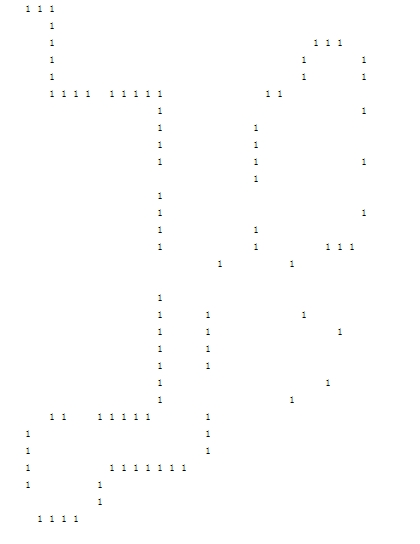
\includegraphics[scale=1]{board.jpg}

\newpage
Graph showing best evolved movement before program got trouble on size controlling (``A" move up, ``$>$" move right, ``V" move down, and ``$<$" move left).\\

\begin{itemize}
\item Best of the ten generations:\\
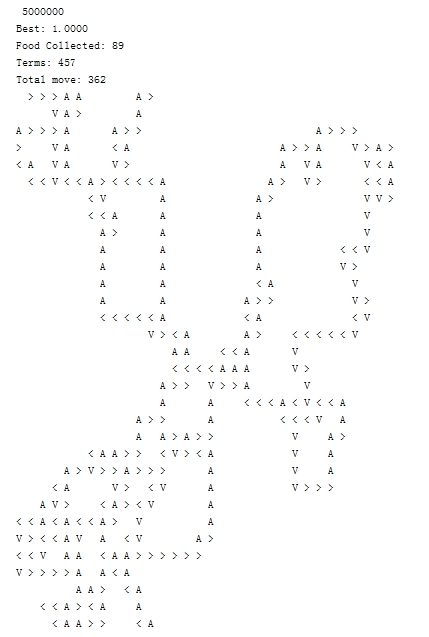
\includegraphics[scale=1]{best2.jpg}
\end{itemize}



\section{Discussion}
\subsection{Ant's generating}
\paragraph{I created my ants by ramped half and half, to make sure the ants will have enough steps to move.}

\subsection{Mutation and Crossover}
\paragraph{The mutation method is desicribed above. Since I have Size control of max depth of 8, the crossover method will check if the children's depth exceeds 8. If one of the children exceed and another not, ignore the bad child and replace one loser by this good child. }

\subsection{Size control and Maximum steps}
\paragraph{Basicly, the Ant should stop until 600 steps or collected all the food, I believe most of my ants don't this requirement. Because of the limitation on max depth, most of my ants has less than 600 terminals, which means the steps will be much less.}

\subsection{Best fitness so far}
\paragraph{The graph shows that my program works well. Although the ant's path to find the food is not perfect, but it at least collected all the food within limited steps. The graph showed above is the only one best path that have all the food collected, others still have several food are not collected.}

\subsection{Improve of the Santa Fe Trail}
\paragraph{The most important thing that needs to be improved is the fitness function. We could add the consideration on total steps, the less step we have, the fitness would be better. }

\end{document}
